%%%%%%%%%%%%%%%%%%%%%%%%%%%%%%%%%%%%%%%%%%%%%%%%%%%%%%%%%%%%%%%%%%%%%%%%%%%%%%%%
\printbibliography%[heading=bibintoc]
\addcontentsline{toc}{chapter}{Bibliography}

% horizontal line
%\vskip\medskipamount
\leaders\vrule width \textwidth\vskip0.4pt % or other desired thickness
\vskip\medskipamount

\noindent All URLs in this thesis have been checked and updated at January 5th
with a script documented at \url{http://tex.stackexchange.com/a/89521/1044}.
The full bibliography is available at \url{http://www.bibsonomy.org/user/voj}. 

\phantomsection
\chapter*{Appendices}
\addcontentsline{toc}{chapter}{Appendices}
\renewcommand{\leftmark}{Appendices}

\appendix
\renewcommand{\thesection}{\Alph{section}}
\renewcommand{\thefigure}{A\arabic{figure}}

\section{Honig's analysis model of data structures}
\label{appendixA}

In his dissertation \textcite{Honig1975} developed an analysis model of data
structures based on a review of 21 programming languages and data base
management systems.  A partial summary of the model is given by
\textcite{Honig1978}.  In Honig's analysis model ``data structures are divided
into three classes (aggregates, associations, and files) and each class is
modeled with a set of questions. Each question delinates one significant
characteristic of the data structure and can be viewed as one axis of a
n-dimensional universe of data structures.'' This appendix includes a copy of
these questions for better comparision, as applied in
section~\ref{sec:honig}.

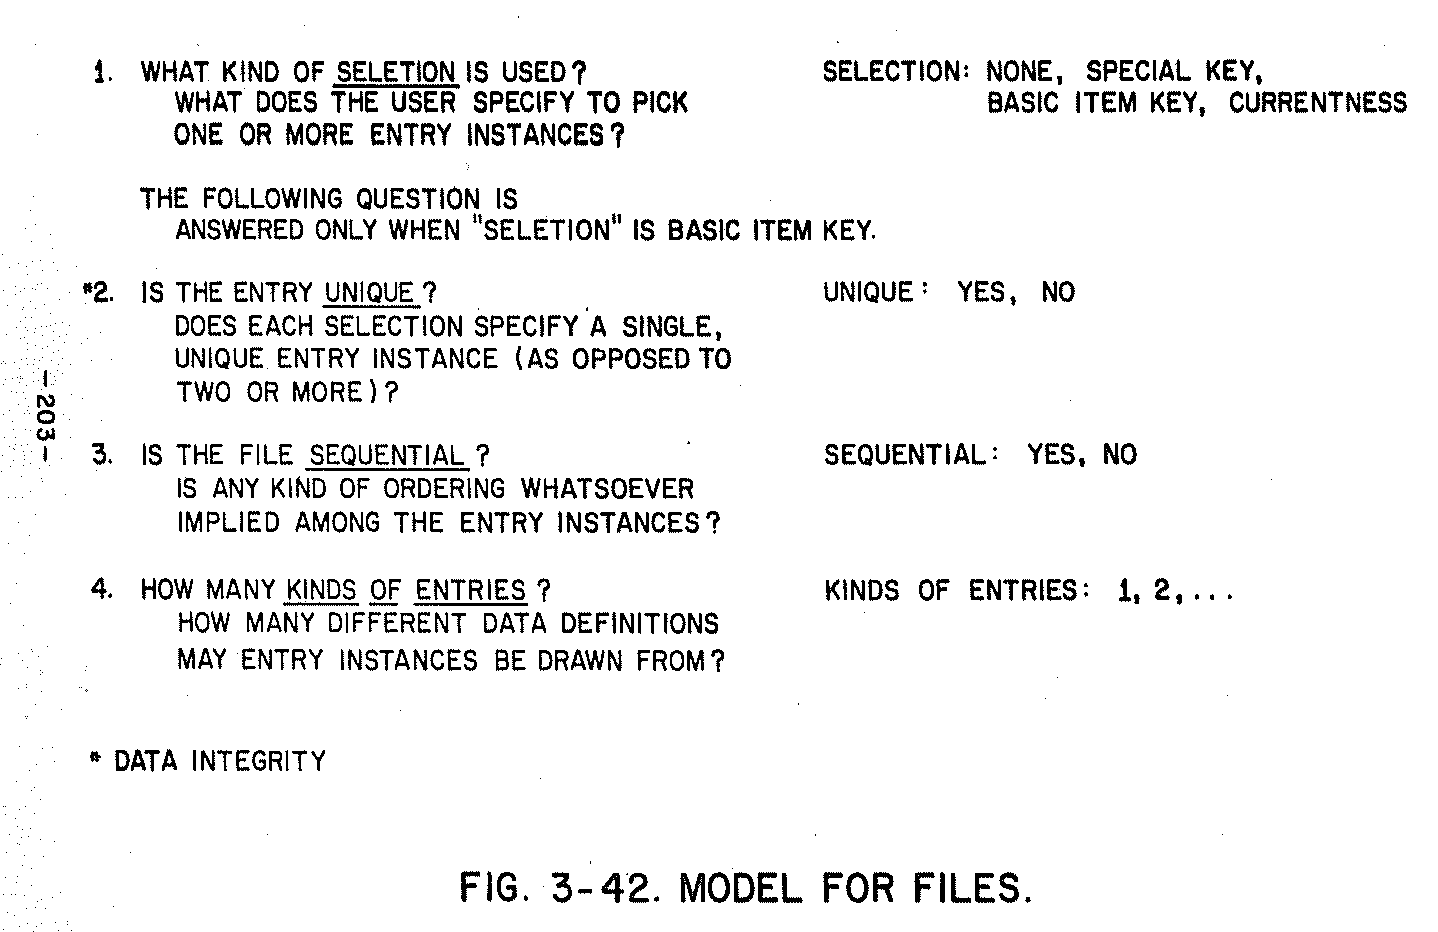
\includegraphics[width=\textwidth]{img/honig1975fig3-42.png}

\thispagestyle{empty}
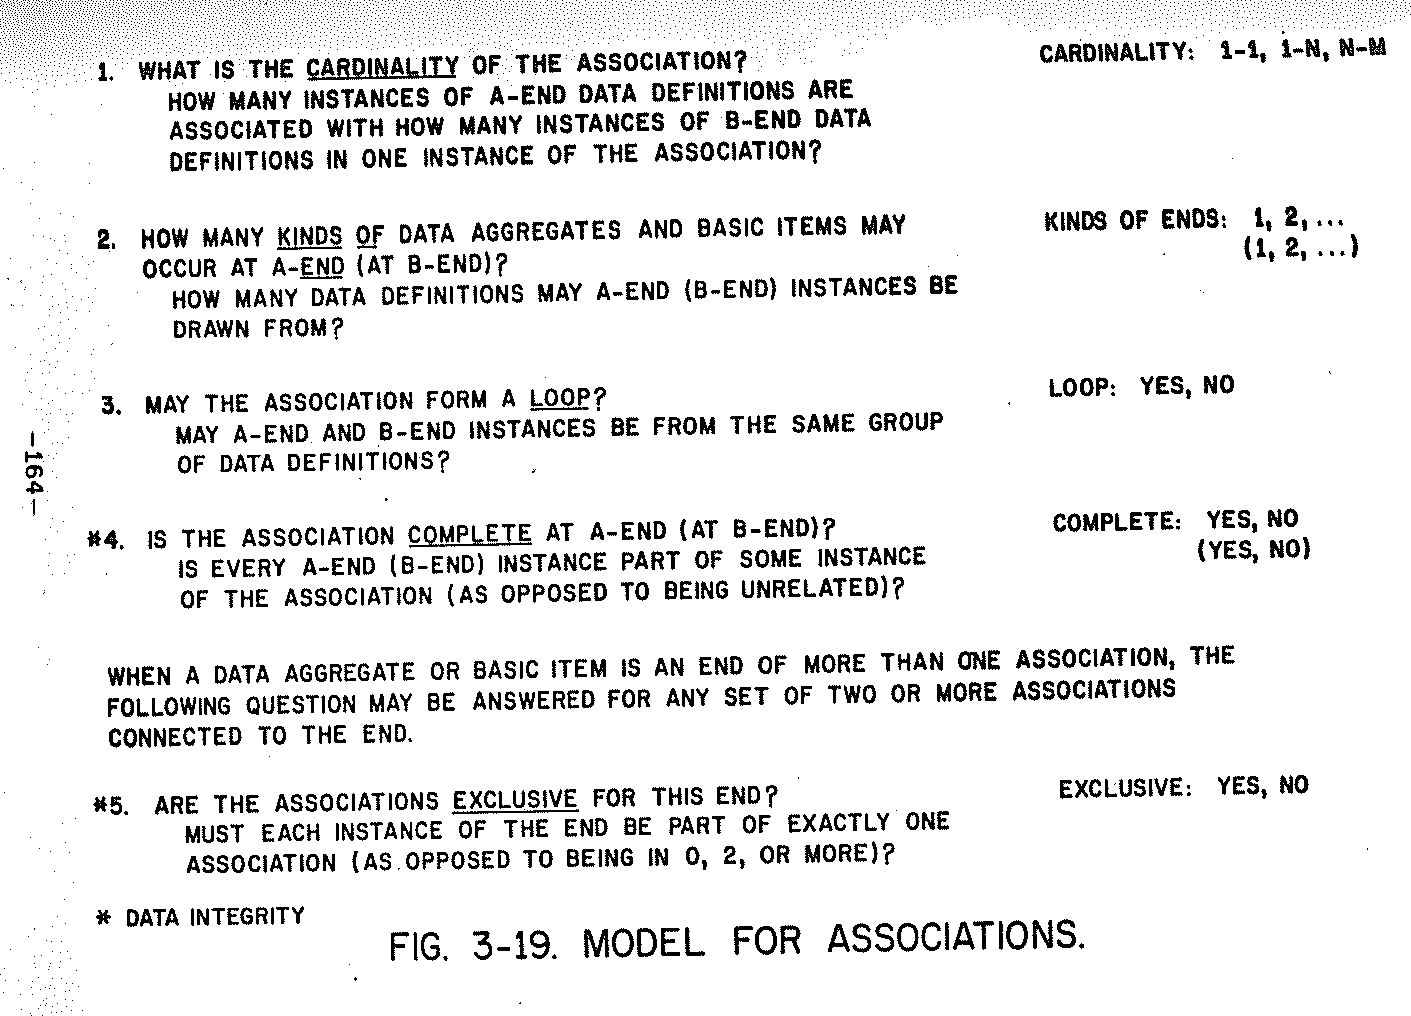
\includegraphics[width=0.9\textwidth]{img/honig1975fig3-19.png}

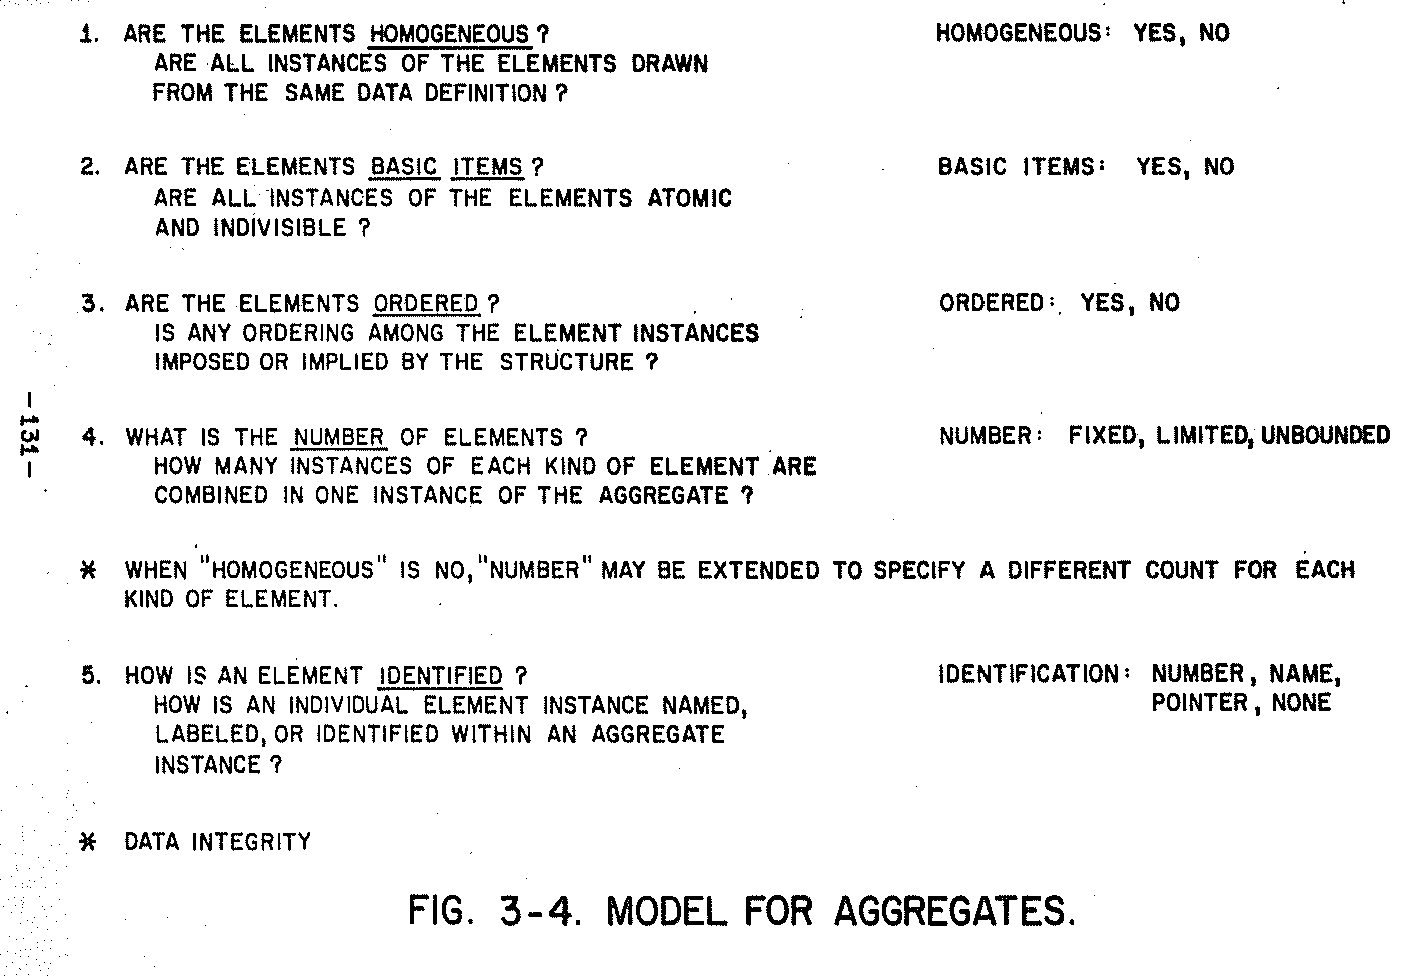
\includegraphics[width=0.9\textwidth]{img/honig1975fig3-4.png}

\clearpage
\section{Conceptual diagrams as digital documents}
\label{appendixB}

The treatment of conceptual diagrams as form of data is not obvious, so it
shall be justified in the following. Figure~\ref{fig:moody2009fig6} is used by
\textcite{Moody2009} to illustrate a specialization of the theory of
communication by \textcite{Shannon1948} to the domain of visual notations:
diagrammatic communication consists of two complementary processes: encoding
and decoding. A diagram (signal) is decoded and encoded using a visual
notation, which defines a set of conventions that both sender and receiver
understand. The diagram can vary by noise, that are minor differences in sizes,
colors, positions etc.  \hspace{5mm}

\begin{figure}[b]
\centering
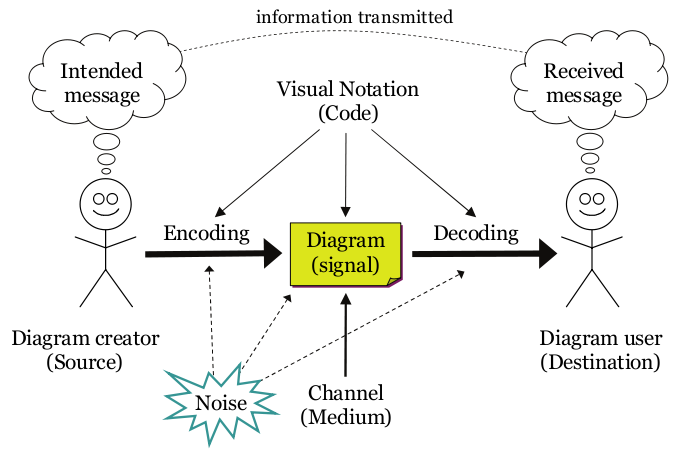
\includegraphics[width=0.7\linewidth]{img/moody2009fig6.png}
\caption{Theory of Diagrammatic Communication as by \textcite{Moody2009}}
\label{fig:moody2009fig6}
\end{figure}

Moody defines the medium (channel) as ``the physical form in which the diagram
is presented (e.g., paper, whiteboard, and computer screen)''. To digitize the
diagram from physical form to digital data, we must identify and encode its
visual symbols and the rules how symbols are combined (see
section~\ref{sec:diagramproperties}). The possibility of such encoding can be
shown by mapping the diagram to another notation, such used in
figure~\ref{fig:moodyvariant}.

\begin{figure}
\centering
\begin{tikzpicture}[
	split/.style={rectangle split, rectangle split parts=2,draw},
	shape2/.style={regular polygon,regular polygon sides=5,draw,minimum width=10mm},
	shape3/.style={ellipse,draw,text width=15mm}]

\node[split,line width=2pt] (signal) {Diagram\nodepart{two}signal};

\node[shape2,left=30mm of signal] (s) {~};
\node[shape2,right=30mm of signal] (d) {~};

\node[split,below=0 of s] (source) {Diagram creator\nodepart{two}Source};
\node[split,below=0 of d] (destination) {Diagram user\nodepart{two}Destination};

\node[shape3,above=0 of s] (im) {Intended message};
\node[shape3,above=0 of d] (rm) {Received message};

\draw[dashed,->] (s) to node[fill=white,name=enc] {Encoding} (signal);
\draw[dashed,->] (signal) to node[fill=white,name=dec] {Decoding} (d);

\draw[out=60,in=120,line width=2pt] (im) to node[fill=white] {information transmitted} (rm);

\node[split,above=8mm of signal] (notation) {Visual Notation\nodepart{two}Code};
\draw[dotted,->] (notation) -> (signal);
\draw[dotted,->] (notation) -> (enc);
\draw[dotted,->] (notation) -> (dec);

\node[split,below=15mm of signal] (channel) {Channel\nodepart{two}Medium};
\draw[ultra thick,->] (channel) -> (signal);

\node[shape=circle,draw,left=4mm of channel] (noise) {noise};
\draw[->] (noise) -> (enc);
\draw[->] (noise) -> (signal);
\draw[->] (noise) -> (dec);

\end{tikzpicture}
\caption{Figure~\ref{fig:moody2009fig6} in different layout}
\label{fig:moodyvariant}
\end{figure}

The readability differs between both diagrams, but they are formally equal, in
the same way as text in different typefaces, size, and layout can be equal if
encoded in \term{Unicode} (see example~\ref{ex:loremipsum}).  Although there is
no Unicode standard for conceptual diagrams, an encoding is possible given a
set of possible visual symbols and combination rules. For this reason
conceptual diagrams can be analyzed as data just like text in Unicode or any
other \term{writing system}.


\vfill

\section{A pattern graph}
\label{appendixC}

Figure~\ref{fig:patterngraph} contains a graph that was automatically created
from the connections between patterns in chapter~\ref{ch:patterns}. Bold arrows
indicate connections to implied patterns or to patterns which occur in the
context of another pattern: for instance the context of a \pattern{separator}
pattern is a \pattern{sequence} and sequences imply an \pattern{embedding}. The
relationship, however, is no formal implication in terms of logic.  Subsets of
this graph are shown in figure~\ref{fig:compatterns} with focus on combining
patterns and figure~\ref{fig:relpatterns} with focus on relational patterns.
The full graph in figure~\ref{fig:patterngraph} further contains dashed arrows
that indicate which patterns can be found in implementations of another
pattern.  One could further draw connections between related patterns, but
these links are too dense to make use of it in a static graph with all
patterns. A hypertext version will be provided at \url{http://aboutdata.org}
for easier browsing of the pattern language. An alternative overview of the
pattern language is given in form of a classification in
table~\ref{tab:patternclassification} at
page~\pageref{tab:patternclassification}.

\begin{sidewaysfigure}
\input{datapatterns/patterngraph}
\caption{Connections between all patterns}
\label{fig:patterngraph}
\end{sidewaysfigure}


\clearpage
% I bet in 40 years
% we will complain about some ancient XML or RDF data that contains strange
% artifacts. Of course MARC is much worse because it is so old, designed for
% cataloging records. But try to get information out of other decade-old
% databases that have been designed for a specific use-case that is not yours,
% and you will stumble upon similar problems.

\section{Deconstruction of a MARC record}
\label{appendixD}

An application of the results of this thesis shall briefly be illustrated with
a fragment of a bibliographic record (figure~\ref{fig:marcrecord}). Similar
analyses of \acro{MARC} have been given by \textcite{Thomale2010} and by
\textcite{Coyle2011}.  The \Tacro{Machine-Readable Cataloging}{MARC} standard
was developed during the 1960s to support library automation in general and to
exchange bibliographic descriptions in particular
\cite{McCallum2009,McCallum2002,Avram1975}.  \acro{MARC} origins in pre-digital
data in form of physical catalog cards --- the format is also criticized for
being suitable only for printing these cards
\cite{Tennant2002,Coyle2005}.\footnote{Sure today's formats will be criticized
in 40 years for not being suitable then.} Nevertheless \acro{MARC} is still
used widely among library systems today .  The brief analysis of the sample
record consists of three steps: first, one needs to clarify the main purpose of
\acro{MARC} to find out what a record actually is.  This is done by means of
the prototype categorization identified in section~\ref{sec:categorization}.
Second, one should ask which basic paradigms have influenced the record
(section~\ref{sec:paradigms}).  And third, one can identify data patterns in
the record (chapter~\ref{ch:patterns}).
% and table~\ref{tab:patternclassification}).

%According to the official \acro{MARC} website \cite{LoC2012}, the ``MARC 21
%Format for Bibliographic Data'' is a standard ``widely used standard{[}s{]}
%for the representation and exchange of bibliographic {[}\ldots{]} information
%data in machine-readable form'' and ``a carrier for bibliographic
%information''.  

On a closer look, \acro{MARC} consists of three methods \cite{LoC2012}: its
\emph{record structure} is used as general data structuring and markup
language, the \emph{content designation} is based on a rough conceptual model
of bibliographic entities (e.g. titles and physical properties), and the actual
\emph{content} of data elements is constrained by cataloging rules
(\acro{ISBD}, \acro{AACR}, \acro{RAK}, \ldots). As neither model nor rules
are defined in a formal language, and many different \acro{MARC} variants and 
interpretations exist, the main use of \acro{MARC} is limited to a
basic record structure (section~\ref{sec:records}), similar to methods
described in section~\ref{sec:dsl} and \ref{sec:markuplanguages}.\footnote{Even
the basic structure cannot be taken for granted: in 2004 German and
Austrian libraries decided to adopt MARC, but they introduced an invalid
subfield code (\texttt{A}), making some of their records broken \acro{MARC}. Such
violating interpretations also occur at schema and conceptual levels.}
Figure~\ref{fig:marcflatmodel} shows a possible model of this structure:
parts may be ordered (\pattern{sequence} pattern) or indexed
(\pattern{identifier} pattern).

\begin{figure}[ht]
\flushright
\begin{tikzpicture}[decoration={brace}]
\matrix (marc) [datamatrix] {
  100 1\#  & |[ucs]| 1F & a & Kernighan, Brian W.         & |[ucs]| 1E ~~ \\
  245 14   & |[ucs]| 1F & a & The C programming language. & |[ucs]| 1E \\
  260 \#\# & |[ucs]| 1F & a & Englewood Cliffs, NJ :      & ~~ ~~\\
           & |[ucs]| 1F & b & Prentice-Hall,              & \\
           & |[ucs]| 1F & c & 1978.                       & |[ucs]| 1E ~~ \\
  700 1\#  & |[ucs]| 1F & a & Ritchie, Dennis M.          & |[ucs]| 1E 1D \\
};
\draw[decorate] 
(marc-6-1.south east) -- node[anchor=north,inner sep=2mm,align=center]
  {field names\\(``tags'')}
(marc-6-1.south west); 
\draw[decorate]
(marc-6-5.south west) -- node[anchor=north,inner sep=2mm,align=center]
  {subfield values} (marc-6-4.south west); 
\draw[decorate] (marc-3-5.north east) -- node[anchor=west,inner sep=2mm]
 {field} (marc-5-5.south east);
\draw[decorate] ($(marc-1-5.north east)+(1cm,0)$) -- 
  node[anchor=west,inner sep=2mm] {record} ($(marc-6-5.south east)+(1cm,0)$);
\draw[<-] (marc-6-3.south) |- +(1em,-2.6em) node[anchor=west] 
{subfield codes as (repeatable) subfield indices};

\end{tikzpicture}
\caption{MARC record and flat file database model with subfields}
% TODO: arrow to "record separator" and "field separator"
\label{fig:marcrecord}
\end{figure}

The governing paradigm of \acro{MARC} is the paradigm of standards and rules
(section~\ref{sec:standardsrules}), so this paradigm can reveal most defects of
the format. It is worth remarking that \acro{MARC} is neither specified by a
formal language nor does it come with a schema language to express subsets and
applications of \acro{MARC} (\acro{MARCXML}, an encoding of \acro{MARC} in
\acro{XML}, only defines a schema for the basic record structure but not for
particular data elements). Furthermore there is no official validator to check
whether records conform to (a specific dialect of) \acro{MARC}.

The lack of formal specifications and automatic tools for validation increase
the importance of intellectual analysis of \acro{MARC} records. Many actual
data patterns do not simply follow the basic record structure of MARC. In
particular \textcite{Thomale2010} found that ``the underlying structure is
based on linguistics rather than a format that was designed to be
machine-readable'', so \acro{MARC} should better be treated like textual
markup. The interpretation of records as markup, which is normally based on
element order (\pattern{sequence}) contrasts with the requirement select data
elements based on the field-subfield-structure (\pattern{identifier} pattern).
For instance one could combine tag, indicator, and subfield code to a
normalized pointer, such as \texttt{245 14 a} for the title in
figure~\ref{fig:marcrecord}.  Within \acro{MARC} fields, \textcite{Coyle2011}
identified three pattern structures: first, subfields can indepedently and
directly describe a resource (so they can be used as part of a pointer).
Second, subfields can qualify or modify other subfields (\pattern{dependence}
pattern or \pattern{flag} pattern), and third, multiple subfields can together
form a resource description (\pattern{sequence}, \pattern{container}, or
\pattern{embedding} pattern). 

An in-depth analysis of \acro{MARC} in particular is out of the scope of this
work, so this appendix ends with some additional pattern instances from the
sample record:

% \texttt{1001\#$\ddagger$a} (identifier): Kernighan, Brian W.

\begin{itemize}
\item The fields 100 and 700 form a \pattern{sequence} of authors.
\item Author names are structured by an \pattern{embedding} with comma as 
  \pattern{separator} (surname, given). Second given names are further abbreviated
  (\pattern{etcetera}).
\item Several instances of punctuation are irrelevant (\pattern{garbage} pattern).
\item \texttt{NJ} in `Englewood Cliffs, NJ' is an \pattern{identifier} that refers 
	to New Jersey.
\item Core elements (`Brian', `Prentice-Hall', \ldots) are instances of
	the \pattern{label} pattern.
\end{itemize}


% time-consuming, intellectual analysis

% it can be encoded in other forms without
% adding conceptual value (for instance in \acro{XML} as \acro{MARCXML}. See
% figure~\ref{fig:jsonrdfxml} for an illustration of similar encodings). A
% \acro{MARC} record is an instance of ISO~2709 (\citeyear{ISO2709:2008}),
% similar to \acro{PICA} (example~\ref{ex:picafieldids}).  In short, a record
% consists of a header (not included in this example) and a list of data fields.
% Each field consists of a field tag, which consists of three digits, an
% indicator, which consists of two lowercase alphanumerical characters or spaces,
% and a list of subfields, each with an alphanumeric subfield code character and
% the actual subfield value.


% conceptual background is rather low, contains schema but many different
% variants. loosely coupled

% Few people have actually read the specification

% Even if there is a standard, people will prefer not to read it, but learn a 
% structure from examples and from the effect of data, when used with a specific
% application --- for instance bibliographic data is primarily shaped not 
% to describe documents, but to nicely print cataloging cards or to trigger 
% the display in electronic catalogs \cite{Tennant2002,Coyle2005,McCallum2009}.
% In practice these applications act as validators of their own interpretation
% of the standard they seem to implement. 

% For practical application: \cite{Thomale2010}
% General LIS: Encyclopedia of Library and Information Sciences


% The record includes punctation from the \tacro{International Standard Bibliographic Description}{ISBD}.

% Schemas (SQL, XML Schema, OWL...) only describe what you
% called "explicit" structure, but as people create data, they add "implicit"
% structure, based on additional conventions or ad-hoc rules.

\begin{figure}
\centering
\begin{tikzpicture}[orm,lpin/.style={label distance=0mm},
  nmrole/.style={roles,unique=2,label=[lpin]above:\ormind{*}}]
\entity (file) at (0,-1) {File};
\entity[right=1.5 of file] (record) {Record} 
       edge[mandatory] node[nmrole] {} (file);
\entity[right=1.5 of record] (field) {Field} 
       edge[mandatory] node[nmrole] {} (record);
\entity[right=1.5 of field] (subfield) {Subfield} 
       edge[mandatory] node[nmrole] {} (field);
\value[right=1.5 of subfield] {Value} 
       edge[mandatory] node[roles,unique] {} (subfield);

\node[rule=*,below=1mm of file.south west,anchor=north west]
  {indexed and/or ordered};
\end{tikzpicture}
\caption{Flat file record model of MARC}
\label{fig:marcflatmodel}
\end{figure}

%\clearpage
%\input{appendixE}

%\chapter*{Index}

% TODO: Separate names, terms, and people
%\textsc{Person}, \textit{Name}, \texttt{data}, \textsl{slanted}
%{\sffamily Language}

%\pagebreak
%\printsubindex[idx]

%\pagebreak
%\printsubindex[person]

%\pagebreak
%\printsubindex[acronym]

\addtocontents{toc}{\protect\vspace{\baselineskip}}% empty line

\clearpage

\begin{otherlanguage}{ngerman}
\unnumberedsection{Danksagung}

Für die fachliche und praktische Unterstützung bei der Vollendung dieser Arbeit
möchte ich mich ausdrücklich bedanken bei
Andreas Krausz,
Brian Ballsun-Stanton,
Ed Summers,
Felix Sasaki,
Gerald Steilen,
Jindřich Mynarz,
Kurt Jansson,
Peter Becker,
Phillip Mayr,
Sally Chambers,
Silvia Czerwinski,
Stefan Gradmann,
Sven Porst,
Till Kinstler,
Thomas Hapke,
Ralph Voß,
Reiner Diedrichs,
Ulrike Reiner,
Viola Voß,
William Honig
sowie den Mitgliedern der Online-Communities Wikipedia und Stack Exchange.

\end{otherlanguage}
